\documentclass[10pt, xcolor=dvipsnames, compress]{beamer}

\usepackage{graphicx}
\usepackage[absolute,overlay]{textpos}
\usepackage{setspace}
\usepackage{caption}
\usepackage{algorithm,algpseudocode}
\usepackage{tikz}

\graphicspath{ {./Images} }

\captionsetup[figure]{font=scriptsize,labelfont=scriptsize}
\captionsetup[table]{font=scriptsize,labelfont=scriptsize}

\title[CNN on FPGA using HLS]{A Convolutional Neural Network (CNN) for handwritten
    digit recognition on FPGA using HLS}
\author[G. Boldini]{Giacomo Boldini\newline\footnotesize giacomo.boldini@studenti.unipr.it}
\institute[UNIPR]{University of Parma\newline
    Master's Degree in Computer Science\newline
    Embedded Systems}
\date{AA 2021/22}

% Justified text.
\renewcommand{\raggedright}{\leftskip=0pt \rightskip=0pt plus 0cm}

% Overlays.
\setbeamercovered{transparent}

\beamertemplatenavigationsymbolsempty

\setbeamerfont{page number in head/foot}{size=\tiny}
\setbeamertemplate{footline}[frame number]

% bibliography

\usepackage[utf8]{inputenc}
\usepackage[english]{babel}
\usepackage[
    style=numeric,
    backend=bibtex,
    sorting=none
    ]{biblatex}
\bibliography{ref}{}
\renewcommand*{\bibfont}{\scriptsize}

% Theme.

\useoutertheme[]{miniframes} % Alternatively: miniframes, infolines, split.
\useinnertheme{circles}

\definecolor{UBCblue}{rgb}{0.04706, 0.13725, 0.26667} % UBC Blue (primary)
\definecolor{UBCgrey}{rgb}{0.3686, 0.5255, 0.6235} % UBC Grey (secondary)
\definecolor{light-grey}{RGB}{240,240,240}

\setbeamercolor{palette primary}{bg=UBCblue,fg=white}
\setbeamercolor{palette secondary}{bg=UBCblue,fg=white}
\setbeamercolor{palette tertiary}{bg=UBCblue,fg=white}
\setbeamercolor{palette quaternary}{bg=UBCblue,fg=white}
\setbeamercolor{structure}{fg=UBCblue} % Itemize, enumerate, etc
\setbeamercolor{section in toc}{fg=UBCblue} % TOC sections
\setbeamercolor{subsection in head/foot}{bg=UBCgrey,fg=white}
\setbeamercolor{title}{bg=UBCblue,fg=white}
\setbeamercolor{block title}{bg=UBCblue,fg=white}
\setbeamercolor{block body}{bg=light-grey, fg=black}
% Grey foreground for slide title.
\setbeamercolor{frametitle}{bg=light-grey,fg=black}


\makeatletter
    \newenvironment{withoutheadline}{
        \setbeamertemplate{headline}[default]
        \def\beamer@entrycode{\vspace*{-\headheight}}
    }{}
\makeatother


\begin{document}

% Line spacing.
\linespread{1.15}

% Title.
\begin{frame}[plain]
    \titlepage
    \begin{textblock*}{5cm}(3.89cm,8cm) % {block width} (coords)
        \centering
        \small
        Project repository here \\ \cite{github-repo}
     \end{textblock*}
\end{frame}

\addtocounter{framenumber}{-1}

% Outline.
\begingroup
\setbeamercolor{palette tertiary}{bg=UBCblue,fg=UBCblue}
\begin{frame}{Goals \& Outline}
    \begin{block}{Goals}

    \begin{itemize}
        \item Creation of a NN for handwritten digit classification.
        \item Implementation of the NN on FPGA using HLS/Vivado.
        \item Prove that HW solutions is faster than SW (C) solutions.
    \end{itemize}

    \end{block}
    \vspace*{2ex}
    {
        \hspace*{-4ex}
        \large
        Outline:
    }
    \tableofcontents

\end{frame}
\endgroup

% PYTHON: TRAIN THE NN MODEL.
\section[Python: NN training]{Python: Create and train NN model}

\begin{frame}{The (C)NN model}

    \textbf{CNN} architecture choosed:
    \begin{itemize}
        \item image-processing task;
        \item no need of manual feature extraction: done automatically;
        \item less number of parameters than other NNs.\\~\
        % With ANN, concrete data points must be provided. For example, in a
        % model where we are trying to distinguish between dogs and cats, the
        % width of the noses and length of the ears must be explicitly provided
        % as data points.
        % When using CNN, these spatial features are extracted from image input.
        % This makes CNN ideal when thousands of features need to be extracted.
        % Instead of having to measure each individual feature, CNN gathers
        % these features on its own.
    \end{itemize}

    %In the end a trade-off was made, choosing an architecture with a low
    %parameter count to be able to have more resources available on the FPGA
    %for parallelization.

    API: Python Keras/Tensorflow \cite*{keras}.\\~\

    Model as simple as possible:
    \begin{center}
        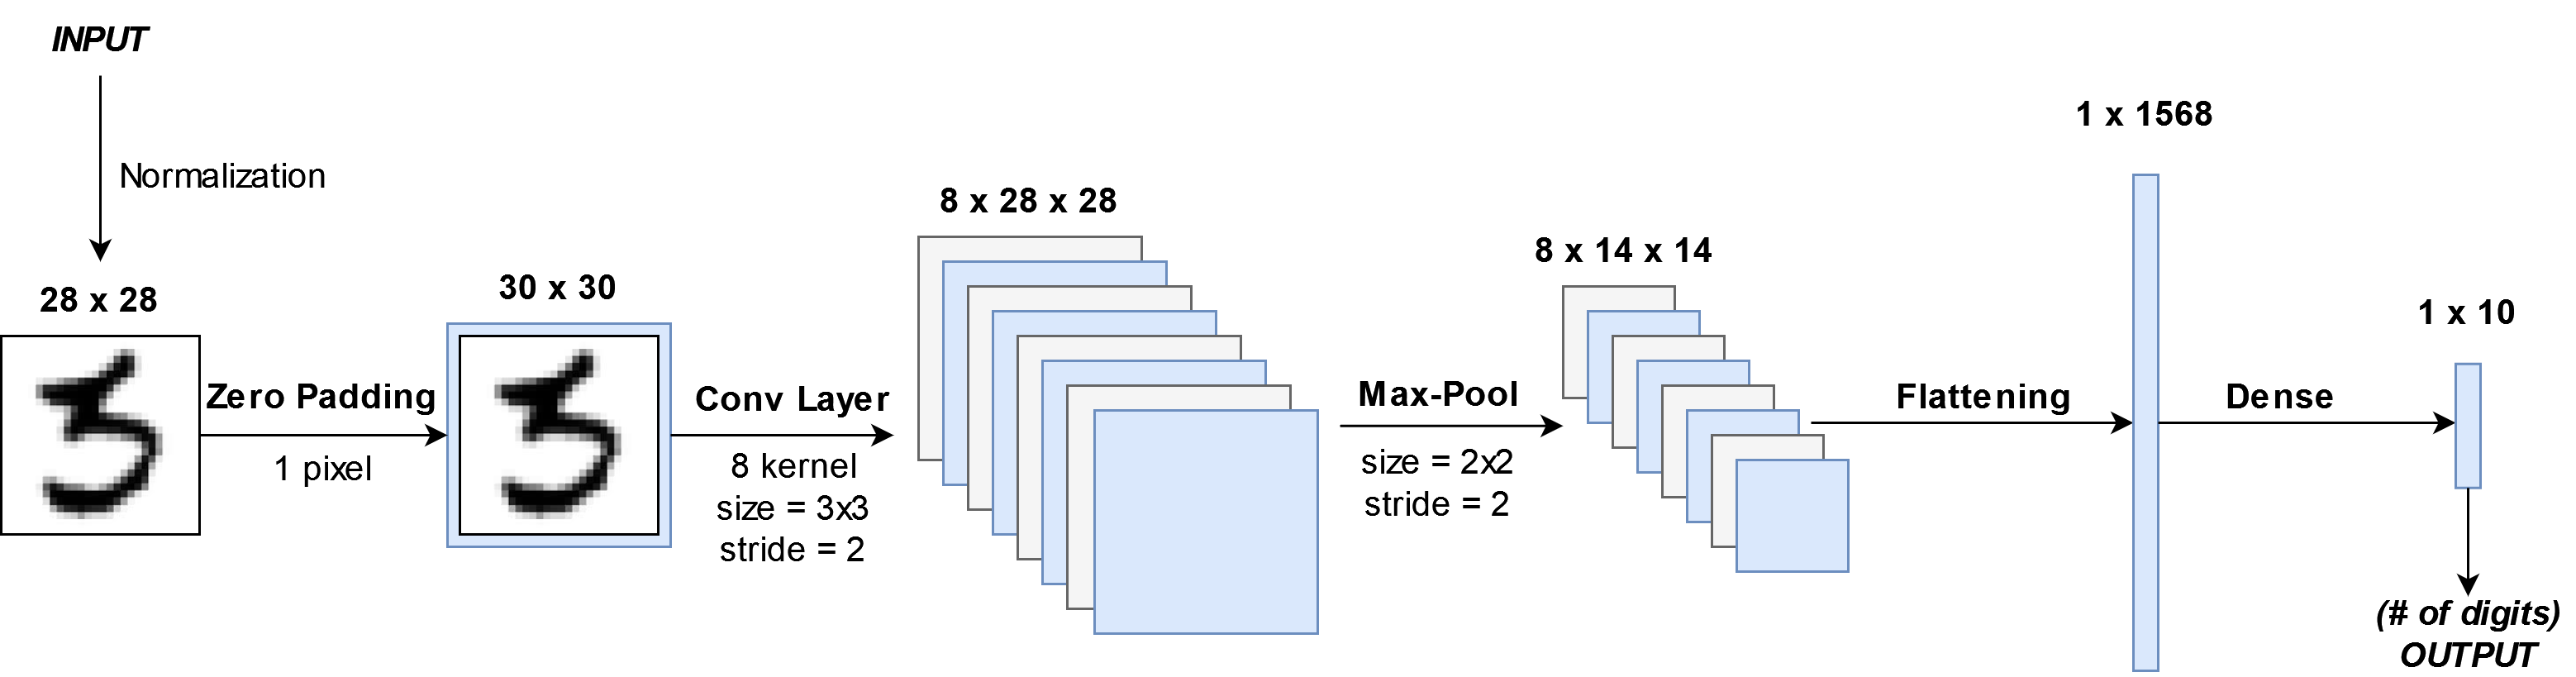
\includegraphics[width=\textwidth]{nndrawio2.png}
    \end{center}

\end{frame}

% \begin{frame}{Other model configurations}
%    Same model but different number of filters:\\~\

%    {
%    \centering
%    \scriptsize
%    \begin{tabular}{lrrrr}
%        \multicolumn{5}{c}{(epochs = 50, validation split = 0.2)} \\
%        filter number & \# param & last val. acc. & test acc. & pred. time (ms) \\
%        \hline
%        \bfseries 8   &  \bfseries 15k     & \bfseries 97.78 & \bfseries 98.07 & \bfseries 36$\sim$38\\
%        16  &   31.5k   & 98.14 & 98.27 & 38 \\
%        32  &   63k     & 98.17 & 98.37 & 38$\sim$40\\
%        64  &   126k    & 98.32 & 98.38 & 38$\sim$40\\~\
%    \end{tabular}

%    }

%    Same model but different number of filters + 1 dense layer:\\~\

%    {
%    \centering
%    \scriptsize
%    \begin{tabular}{lrrrr}
%        \multicolumn{5}{c}{(epochs = 50, validation split = 0.2)} \\
%        filter number & \# param & last val. acc. & test acc. & pred. time (ms) \\
%        \hline
%        8   &   158k    & 92.67 & 93.18 & 38\\
%        16  &   315k    & 93.80 & 93.42 & 50\\
%        32  &   630k    & 94.98 & 95.05 & 50\\
%        64  &   1256k   & 94.73 & 94.23 & 52\\~\
%    \end{tabular}

%    }

% \end{frame}

\begin{frame}{Training}

\begin{columns}[T]
    \begin{column}{.6\textwidth}

        TrainX shape = (60000, 28, 28)\\
        Training epochs = 10 (empiric)\\~\

        Layers' trainable parameters:\\~\

        {
        \tiny
        \begin{tabular}{lll}
            Layer (type) & Output Shape & Param \# \\
            \hline
            ZeroPadding2D & (30, 30, 1) & 0 \\
            Conv2D & (28, 28, 8) & 80 \\
            MaxPooling2D & (14, 14, 8) & 0 \\
            Flatten & (1568) & 0 \\
            Dense & (10) & 15690 \\
            \hline
            TOT &  & \textbf{15770} \\~\

        \end{tabular}
        }

        Accuracy:
        \begin{itemize}
            \item validation set (20\% of test set): 97.78\%
            \item test set (\#10000 samples): \textbf{98.070\%}\\~\
        \end{itemize}

        %Accuracy on test set: 97.760

        Mean time for a prediction: \textbf{$\sim$35 ms}
    \end{column}
    \begin{column}{.4\textwidth}
        Training history:\\
        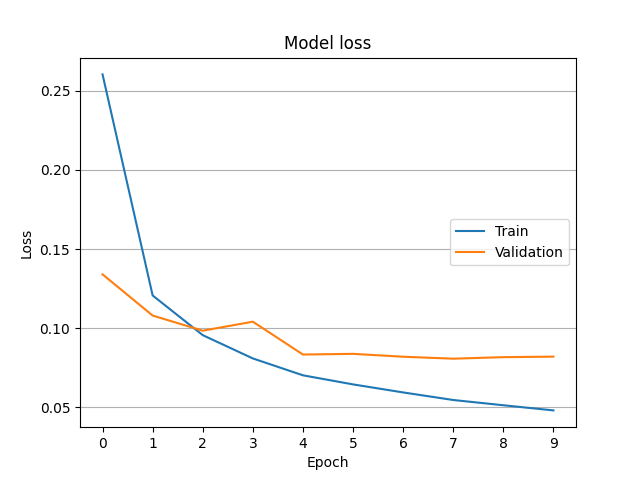
\includegraphics[width=\textwidth]{history_loss_8.png}
        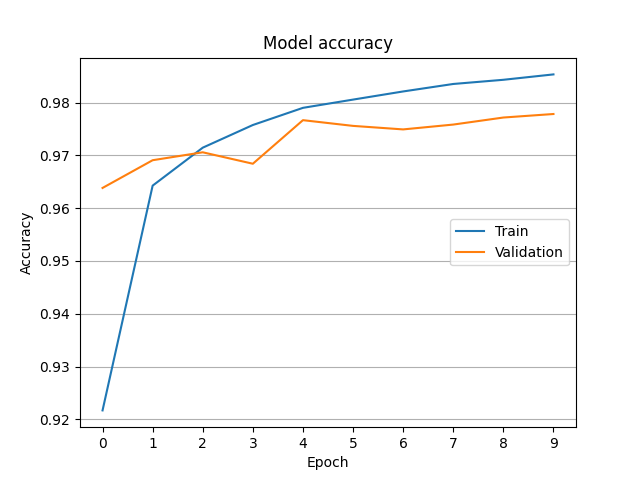
\includegraphics[width=\textwidth]{history_accuracy_8.png}

    \end{column}
\end{columns}


\end{frame}

% C: NN implementation.
\section[C: NN implementation]{C: NN implementation}

\begin{frame}{C \texttt{cnn()} function}

    % \begin{algorithmic}[1]
    %    \Procedure{Recursion}{$a$}
    %        \State $a\gets\Call{Recursion}(a)$ \Comment{Call Recursion again}
    %        \State \textbf{return} $a$
    %    \EndProcedure
    %    \STATE void cnn(float img\_in [IMG\_ROWS][IMG\_COLS], float prediction[DIGITS])
    %    %\FOR{$i=1$ to $N$}
    %    %\FOR{$j=1$ to $JJJJ$}
    %    %\STATE $energy[i*JJJ+j] =$
    %    %$ interpolate(AAA[i*JJJ+j], ZZZ)$
    %    %\ENDFOR
    %    %\ENDFOR
    % \end{algorithmic}

    % \hspace{-.8em}

    {
        \ttfamily
        \footnotesize
        void \textbf{cnn}(float img\_in [IMG\_ROWS][IMG\_COLS], float prediction[DIGITS])\\
        \{ \\
        \hspace*{1em}// Normalization and padding.\\
        \hspace*{1em}float pad\_img [PAD\_IMG\_ROWS][PAD\_IMG\_COLS] = \{ 0 \};\\
        \hspace*{1em}\textbf{normalization\_and\_padding}(img\_in, pad\_img);\\
        \hspace*{1em}// Convolution.\\
        \hspace*{1em}float features [FILTERS][IMG\_ROWS][IMG\_COLS] = \{ 0 \};\\
        \hspace*{1em}\textbf{convolutional\_layer}(pad\_img, features);\\
        \hspace*{1em}// Pooling.\\
        \hspace*{1em}float pool\_features [FILTERS][POOL\_IMG\_ROWS][POOL\_IMG\_COLS] = \{ 0 \};\\
        \hspace*{1em}\textbf{max\_pooling\_layer}(features, pool\_features);\\
        \hspace*{1em}// Flattening.\\
        \hspace*{1em}float flat\_array [FLAT\_SIZE] = \{ 0 \};\\
        \hspace*{1em}\textbf{flattening\_layer}(pool\_features, flat\_array);\\
        \hspace*{1em}// Dense.\\
        \hspace*{1em}\textbf{dense\_layer}(flat\_array, prediction);\\
        \} \\
    }

\end{frame}


\begin{frame}{C \texttt{main()} / testbench}

    \begin{center}
        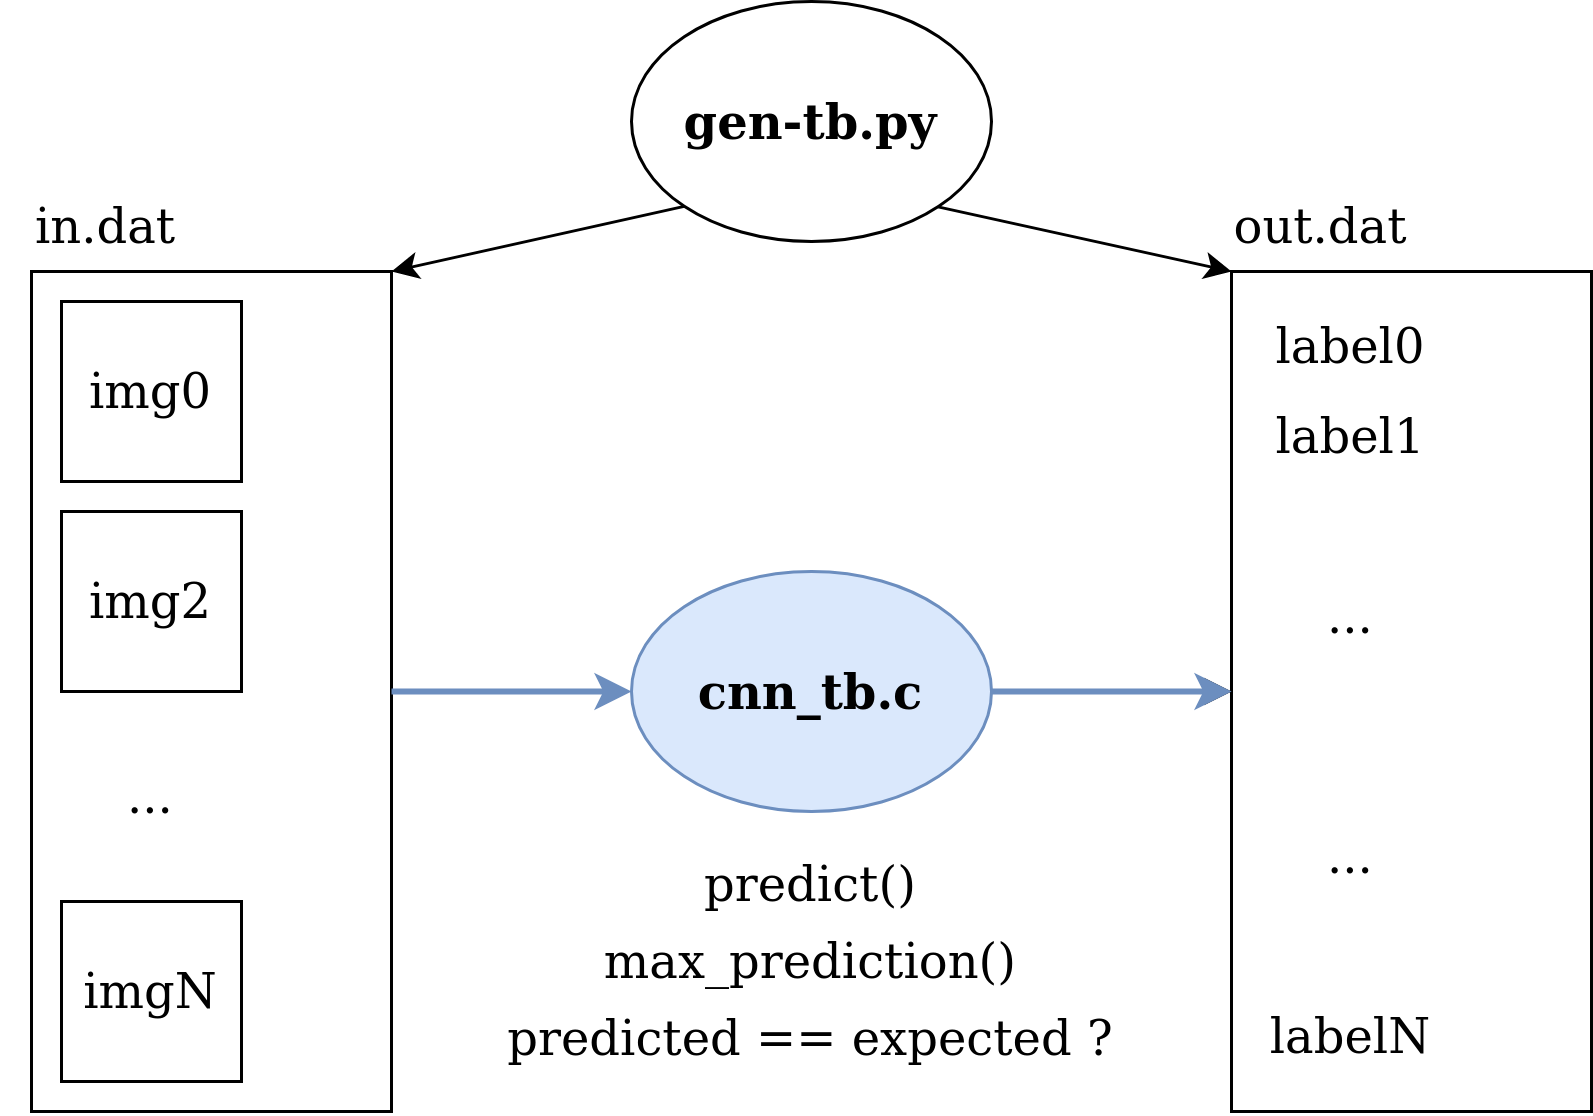
\includegraphics[width=.4\textwidth]{tb.png}
    \end{center}

    \vspace{.5em}

    \begin{columns}[T]
        \begin{column}{.5\textwidth}
            \begin{itemize}
            \item MNIST TestX samples: 10000\\
            \item Accuracy: $\frac{\text{correct predictions}}{\text{total predictions}}$
            \end{itemize}


        \end{column}
        \begin{column}{.5\textwidth}
            \begin{itemize}{}
                \item[]\hspace{-2em} N: 100 $\thicksim$ 250\\
                \item[]\hspace{-2em} Test successfull $\Leftrightarrow$ Accuracy $\ge$ 95\%
            \end{itemize}

        \end{column}
    \end{columns}
    \vspace{1.5em}

    Mean time for a prediction:
    \begin{itemize}
        \item \textbf{0.82 ms} - O0 ($\sim$40x faster than Python)
        \item \textbf{0.17 ms} - O3 ($\sim$200x faster than Python)
    \end{itemize}

\end{frame}


% Vitis/C++: NN synthesis.
\section[Vitis/C++]{Vitis/C++: NN synthesis and validation}


\begin{frame}{Code optimizations for Vitis/FPGA}

    C implementation not optimized for Vitis/FPGA deployment.
    \vspace{1.5ex}


    \begin{block}{CNN parallelism}
        \begin{enumerate}
            \item CNN creates implicit parallelism on filters.
            \item CNN does not need all the data from the previous layer to start
            computing the output response for the current layer.
        \end{enumerate}

    \end{block}


    % \vspace{1.5ex}
    % \begin{itemize}
    %     \item data input/output with std array;
    %     % \item fixed point arytmethic?
    %     \item does not create/support parallelism (dataflow).
    % \end{itemize}
    \vspace{1.5ex}


    Optimize code:
    \begin{itemize}
        \item \texttt{hls::stream} \cite{stream} between functions:
        % \hspace*{2em}
        FIFO with blocking API \texttt{read()} and \texttt{write()}.\\
        \begin{enumerate}
            \item + new function \texttt{dataflow\_section(img1,img2,\dots,img8)}
            that clones input image \texttt{FILTER\_NUMBER} times.
            \item + sw chages: eg. convolution with sliding-window.
        \end{enumerate}

    \end{itemize}

\end{frame}

\begin{frame}{C simulation}
    Total predictions: 500.\\
    Correct predictions: 98.20 \% \hspace*{1em} $\rightarrow$ \textbf{OK}.\\
    Average latency: 2.33 ms \hspace*{1em} $\rightarrow$ a little bit
        more than C.\\~\

    Some bad classifications:

    {\scriptsize (images normalized and rounded)}\\[2ex]

    \begin{spacing}{0.9}
    \begin{columns}[T]
        \begin{column}{.15\textwidth}
            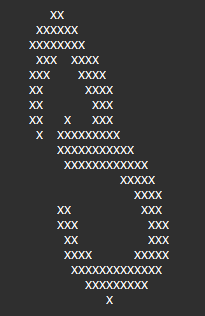
\includegraphics[width=\textwidth]{3-bad-class.png}
        \end{column}
        \begin{column}{.15\textwidth}
            \scriptsize
            Expected: \textbf{3}\\[2ex] Got:\\
            0: 0.000002\\
            1: 0.000000\\
            2: 0.001373\\
            3: 0.213332\\
            4: 0.000003\\
            5: 0.000935\\
            6: 0.000000\\
            7: 0.000000\\
            8: 0.783027\\
            9: 0.001329

        \end{column}
        \begin{column}{.01\textwidth}
            \rule{.1mm}{0.4\textheight}
        \end{column}

        \begin{column}{.15\textwidth}
            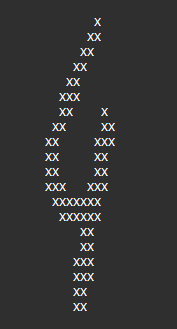
\includegraphics[width=.85\textwidth]{4-bad-class.png}
        \end{column}
        \begin{column}{.15\textwidth}
            \scriptsize
            Expected: \textbf{4}\\[2ex]
            Got:\\
            0: 0.000000\\
            1: 0.000045\\
            2: 0.000020\\
            3: 0.000661\\
            4: 0.253086\\
            5: 0.000059\\
            6: 0.000414\\
            7: 0.000036\\
            8: 0.000321\\
            9: 0.745357
        \end{column}

        \begin{column}{.01\textwidth}
            \rule{.1mm}{0.4\textheight}
        \end{column}

        \begin{column}{.15\textwidth}
            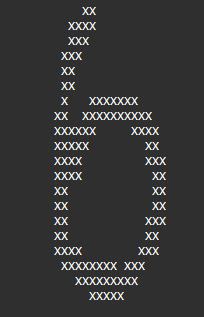
\includegraphics[width=\textwidth]{6-bad-class.png}
        \end{column}
        \begin{column}{.15\textwidth}
            \scriptsize
            Expected: \textbf{6}\\[2ex]
            Got:\\
            0: 0.735325\\
            1: 0.000000\\
            2: 0.000000\\
            3: 0.000000\\
            4: 0.000000\\
            5: 0.000019\\
            6: 0.264633\\
            7: 0.000000\\
            8: 0.000004\\
            9: 0.000020

        \end{column}

    \end{columns}
    \end{spacing}
\end{frame}

\begin{frame}[allowframebreaks]{C synthesis}
    Common parameters:
    \begin{itemize}
        \item Target device: \textbf{xc7a200tfbg484-1}
        \item Target clock period: \textbf{10ns} (clock freq.: 100 $MHz$)\\~\
    \end{itemize}

    Different \textit{"levels of optimization"} (directives):

    \begin{enumerate}
        \item No directives\\~\

        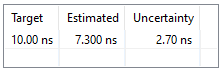
\includegraphics[width=.2\textwidth]{Synthesis-result/no_opt_timing.png}
        \linebreak
        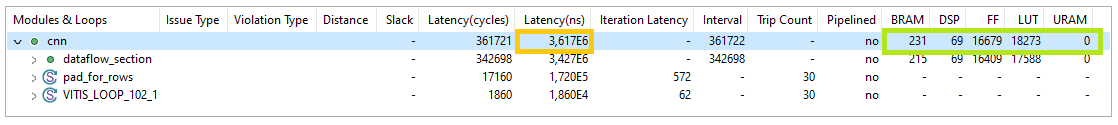
\includegraphics[width=\textwidth]{Synthesis-result/no_opt.png}

    \framebreak
        \item Default directives\\~\


        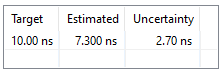
\includegraphics[width=.2\textwidth]{Synthesis-result/opt_def_timing.png}
        \linebreak
        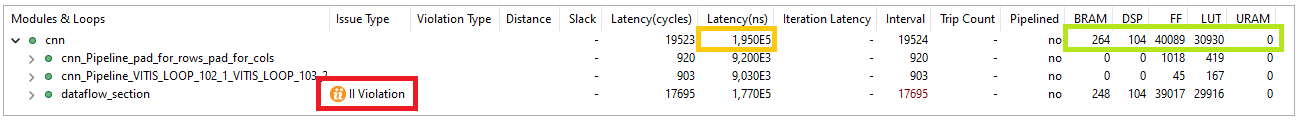
\includegraphics[width=\textwidth]{Synthesis-result/opt_def.png}

        % \begin{itemize}
        %    \item Some memory dependency violation due to default pipelining.
        % \end{itemize}

        \item Dataflow directive\\~\

        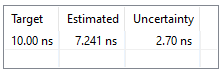
\includegraphics[width=.2\textwidth]{Synthesis-result/opt_full_timing.png}
        \linebreak
        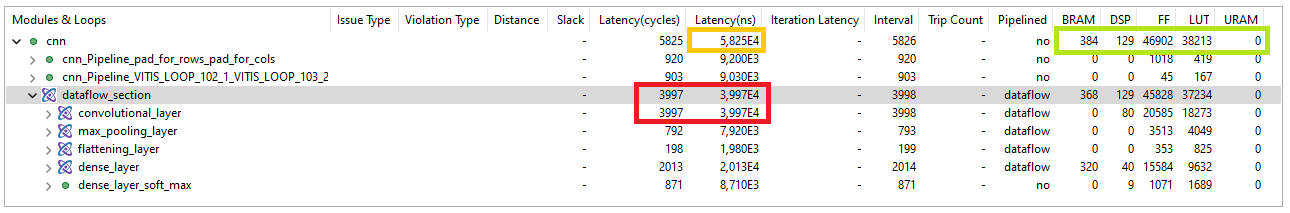
\includegraphics[width=\textwidth]{Synthesis-result/opt_full_detail.png}

        % \begin{itemize}
        %    \item No more violation;
        %    \item Dataflow_section: max = total time --> parallelism
        % \end{itemize}
    \framebreak
        Dataflow view:
        \begin{center}
            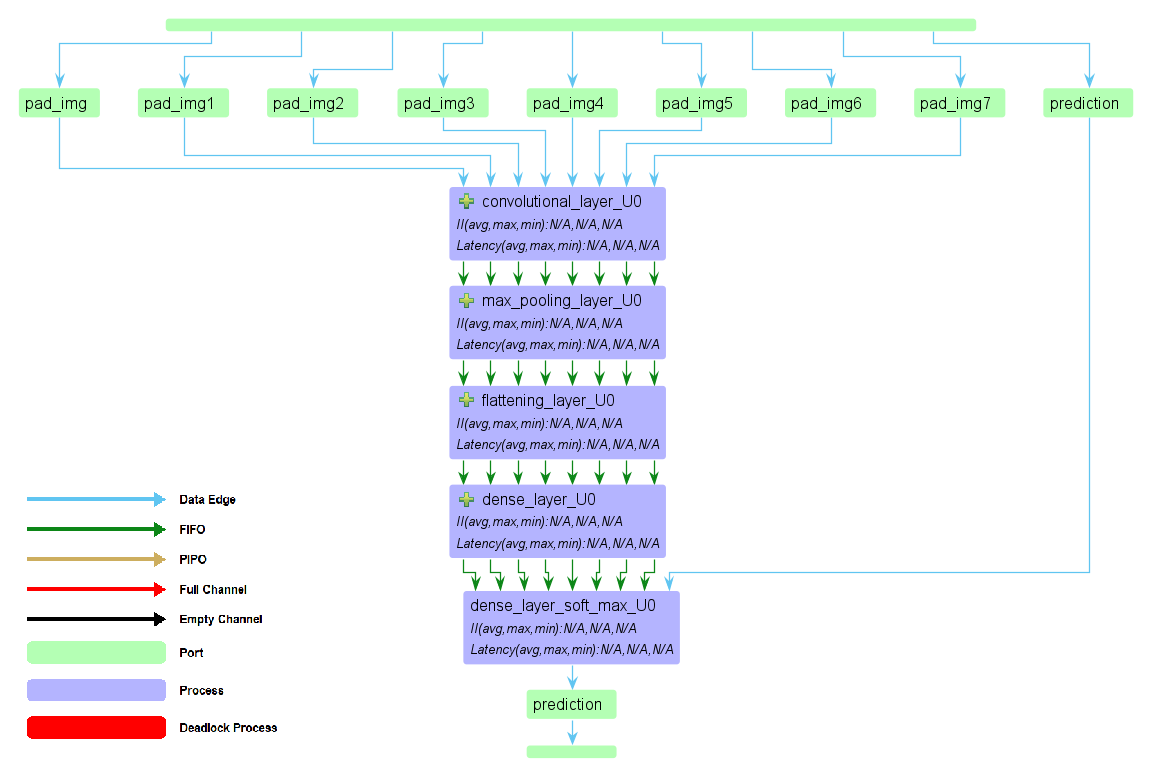
\includegraphics[width=.58\textwidth]{dataflow-view.png}
        \end{center}
        \tiny{(zoom on convolutional\_layer)}
        \begin{center}
            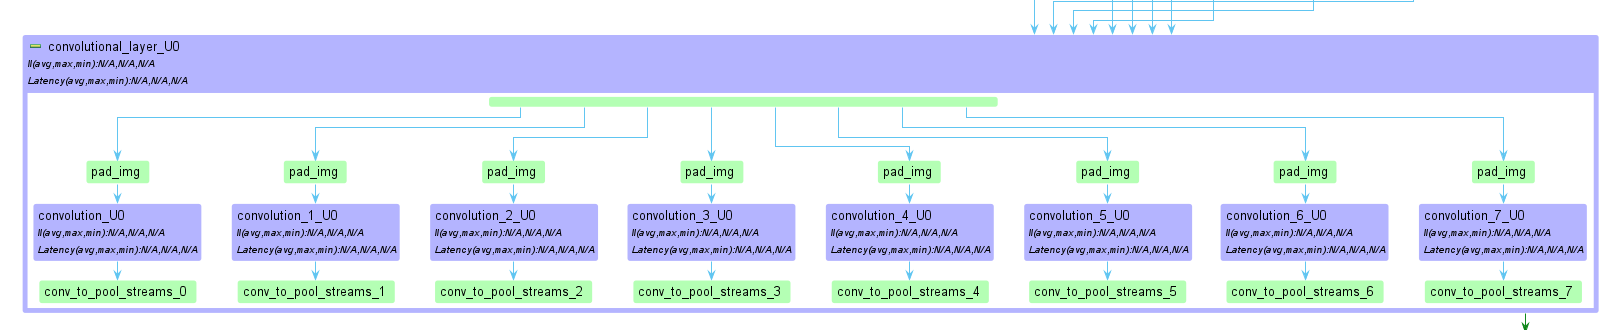
\includegraphics[width=.76\textwidth]{dataflow-view-zoom.png}
        \end{center}

    \end{enumerate}
\end{frame}


\begin{frame}{Validation and implementation}

    \hspace*{-2.2em} C/RTL Cosimulation $\rightarrow$ \textbf{OK}

    \vspace*{.5em}
    \begin{columns}[T]
        \begin{column}{.6\textwidth}
            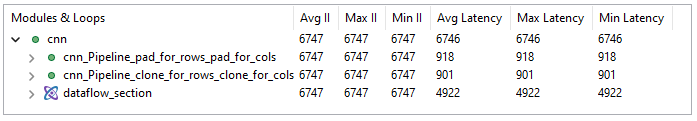
\includegraphics[width=\textwidth]{Synthesis-result/co_simulation.png}\\
            $\rightarrow$ prediction time: \textbf{0.067} ms
        \end{column}

        \begin{column}{.4\textwidth}


        {
            \ttfamily
            \tiny
            \linespread{1}
            Total predictions: 100\\
            Correct predictions: 99.00 \%\\
            Average latency: 0.290000 (ms)\\
            *** C/RTL co-simulation finished: PASS ***\\


        }

        \end{column}

    \end{columns}


    \vspace*{1em}

    \hspace*{-2.2em} Implementation (Vivado)

    \vspace*{.5em}

    % {
    %    \tiny
    %    \ttfamily
    %    \#=== Post-Synthesis Resource usage ===\\
    %    SLICE:            0\\
    %    LUT:          28929\\
    %    FF:           38357\\
    %    DSP:            129\\
    %    BRAM:           224\\
    %    URAM:             0\\
    %    LATCH:            0\\
    %    SRL:           1933\\
    %    CLB:              0\\

    %    \#=== Final timing ===\\
    %    CP required:                     10.000\\
    %    CP achieved post-synthesis:      8.123\\
    %    Timing met
    % }
    \begin{columns}
        \begin{column}{\textwidth}
            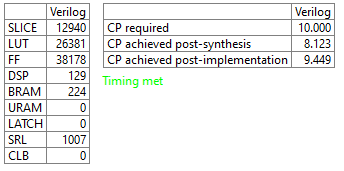
\includegraphics[width=.6\textwidth]{impl.png}\\

        \end{column}
    \end{columns}
    % 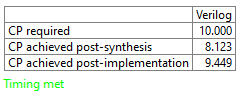
\includegraphics[width=.3\textwidth]{impl1.png}

    \begin{tikzpicture}[remember picture,overlay]
        \node[xshift=-7em,yshift=-22em] at (current page.north east){%
        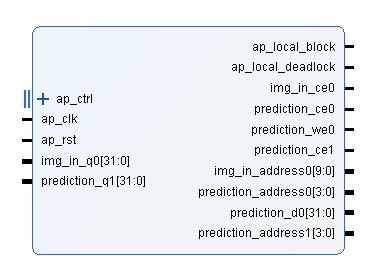
\includegraphics[width=.4\textwidth]{module-cnn.png}};
    \end{tikzpicture}

\end{frame}

% \begin{frame}{Changing the board and the clock}

%    Relaxing the clock (10 $\sim $ 20 ns):\\

%    \begin{itemize}
%        \item[$\rightarrow$] No improvements. \\~\
%    \end{itemize}



%    Changing the boards:\\~\

%    {
%        \tiny
%        \begin{tabular}{@{\extracolsep{4pt}}lrrrrrrrrr@{}}
%            & \multicolumn{3}{c}{timing (ns)} & \multicolumn{6}{c}{performance}\\
%            \cline{2-4}
%            \cline{5-10}
%            board & target & estim & uncert & lat (cycl) & lat (ns) & BRAM & DSP & FF & LUT \\
%            \hline
%            xc7a200t-fgg484-1 & 10 & 7.241 & 2.7 & 3825 & 3.825e4 & 384 & 129 & 46902 & 38213 \\
%            xc7a100t-fgg484-1 & 10 & 7.241 & 2.7 & 3825 & 3.825e4 & 384 & 129 & 46902 & 38213 \\
%            xc7a75t-fgg484-1 & 10 & 7.241 & 2.7 & 3825 & 3.825e4 & 384 & 129 & 46902 & 38213 \\

%            From 100 to 25 the resource are too limited for cnn.

%        \end{tabular}
%    }


%        %\begin{itemize}
%            %\item xc7a200t (\textbf{actual}) $\sim$ € 300
%                %\item xc7a100t (\textbf{actual}) $\sim$ € 150

%                %clock required:
%            %\end{itemize}

% \end{frame}

% \begin{frame}{Validate synthesis results (C/RTL co-simulation)}
% \end{frame}

\section{Conclusions}

\begin{frame}{Conclusions}
    Main goal reached: \textbf{HW faster than SW - but not always}.
    \begin{center}
        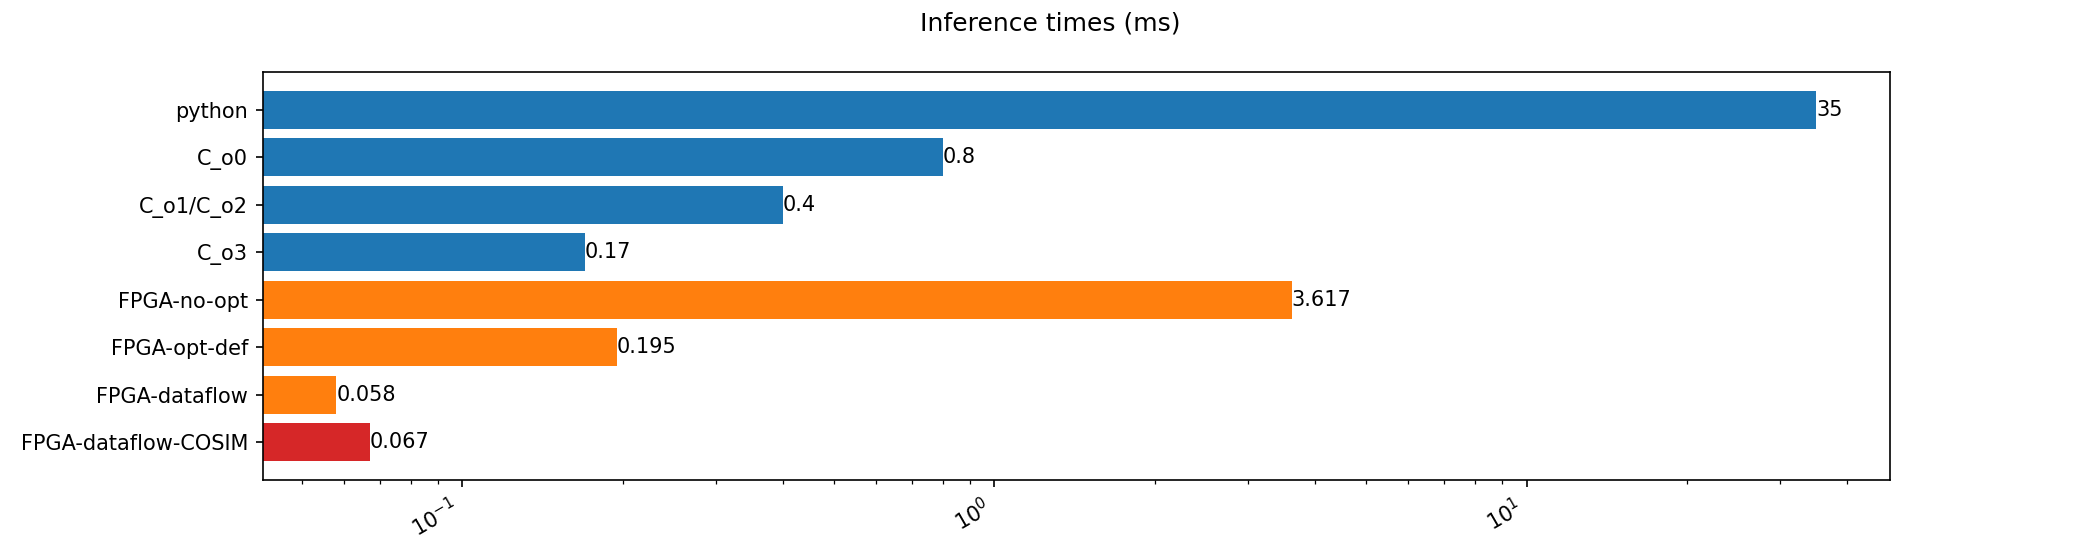
\includegraphics[width=.8\textwidth]{times.png}
    \end{center}

    As future works:
    \begin{itemize}
        \item small SW changes could improve parallelism;
        \item more targeted Vitis pragmas could improve performance;
        \item using \textit{fixed-point} arithmetic could reduce area
        \textbf{(* performance too)};
        \item \texttt{grid-search} on NN architecture could increase accuracy
        (more performance) and reduce FPGA area (less price).
    \end{itemize}

    % \textbf{Datasets}, to have well-formed summaries:
    % \begin{itemize}
    %    \item More constraints;
    %    \item Less noise.
    % \end{itemize}
    % \pause
    % \textbf{Evaluation protocol (ROUGE)}:
    % \begin{itemize}
    %    \item Weakly correlated to human judgments;
    %    \item Fail to evaluate critical features (such as \textit{factual correctness}).
    % \end{itemize}
    % \pause
    % \textbf{Models}:
    % \begin{itemize}
    %    \item Rely too heavily on layout bias;
    %    \item Offer limited diversity in their outputs.
    % \end{itemize}

\end{frame}

\appendix

\begingroup
\setbeamercolor{palette tertiary}{bg=UBCblue,fg=UBCblue}
\setbeamertemplate{footline}{}

\nocite{*}
\begin{frame}[noframenumbering]{}
    % \fontsize{3}{6}\selectfont
    \huge
    Thank you for your attention.\\[4ex]

    \large
    References

    \printbibliography
\end{frame}

\endgroup

% \begin{frame}{Solution 0: no directive}
%    \begin{itemize}
%        \item Sythesis:

%        \begin{tabular}{l}
%            timing \\
%            \hline
%            latency \\
%            \hline
%            utilization \\
%        \end{tabular}



%        \item C/RTL Simulation: \textbf{OK}
%        latency: 1.76 ms

%        \item Implementation (Vivado):

%    \end{itemize}
% \end{frame}

% \begin{frame}{Solution 1: default directives}
%    \begin{itemize}
%        \item Automatic pipeline of loops
%        \item Some warning/violation: resource limitation / memory dependency\\
%                (disappear with DATAFLOW?)
%        \item Slack -0.58
%    \end{itemize}

% \end{frame}

% \begin{frame}{Solution 2: dataflow}
%    Slack: -0.58\\
%    incremento il periodo di clock
% \end{frame}

\end{document}
